\section{Pianificazione}\label{piana}
Le fasi individuate nella sezione \ref{divisioneFasi} contengono al loro interno diverse attività, queste possono essere eseguite in parallelo qualora non esistano tra esse delle dipendenze temporali. \\
Le attività di ogni fase sono state a loro volta suddivise in sottoattività in modo da poter esser associate ad una o più risorse.
%sono state suddivise in attività, le quali sono state suddivise a loro volta in sotto-attività in modo da poter essere associate ad una o più risorse.\\
La scelta di scindere le attività sottoattività, oltre a permettere un controllo a grana più fine sulle risorse, consente di aver un maggior controllo del tempo disponibile. \\
In questo modo sarà possibile applicare PDCA aumentando quindi l'efficienza e l'efficacia del \gloxy{team} nei processi ripetibili. \\
Per ogni fase viene riportato il relativo \gloxy{diagramma di Gantt} con la pianificazione delle sottoattività e la \gloxy{milestone} che sancisce il termine della fase.
\subsection{\fAt}
\textbf{Periodo:} dal 2014-12-01 al 2015-01-23 \\
Questa prima fase inizia il 2014-12-01 e termina con la consegna dei documenti necessari alla \RR. \\
Lo scopo di questa fase è analizzare il problema per definire in modo chiaro e non ambiguo i requisiti. Oltre al documento di \AR vengono redatti tutti i documenti di supporto, necessari alle attività di sviluppo. \\
Durante questa fase vengono svolte le seguenti attività:
\begin{itemize}
\item \textbf{Norme di \gloxy{progetto}:} gli \rAPs organizzano l'ambiente di lavoro definendo gli strumenti e le regole che saranno adottate nella realizzazione del \gloxy{progetto}. Tutto ciò verrà formalizzato nelle \NP;
\item \textbf{Studio di Fattibilità:} vengono analizzati i vari capitolati proposti al fine di scegliere il \gloxy{progetto} da realizzare. Il capitolato scelto e i motivi della scelta vengono riportati nello \SF;
\item \textbf{Piano di \gloxy{Progetto}:} il \rRP, basandosi sulle date a disposizione, pianifica il lavoro e redige il \PP;
\item \textbf{Piano di Qualifica:} Gli \rAs in collaborazione con gli \rAPs e il \rRP, redigono il \PQ;
\item \textbf{Analisi dei Requisti:} gli \rAs iniziano a stendere una prima versione dell'\AR;
\item \textbf{Glossario:} viene redatta una prima versione del \G.
\end{itemize}
\subsubsection{Diagramma di Gantt delle attività}
\begin{landscape}
\begin{figure}[h]
\centering
%\includegraphics[width=23cm,height=13cm]{../immagini/gantt/GanttFaseAnalisi.png}\textwidth
%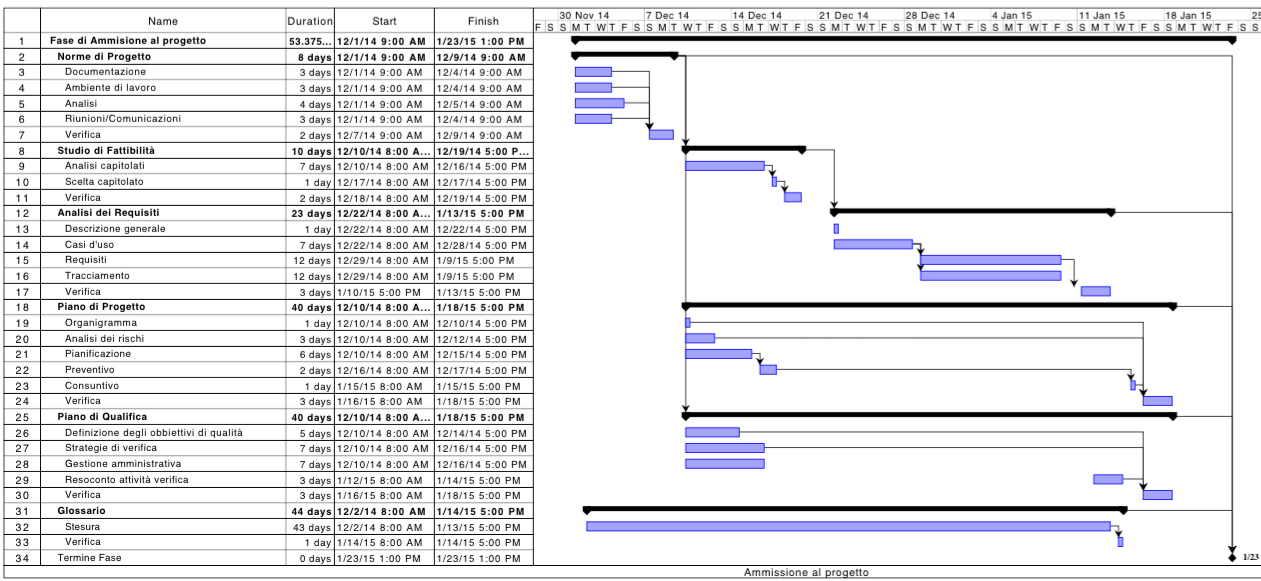
\includegraphics[width=\textwidth,keepaspectratio]{../immagini/gantt/ammissioneP.png}
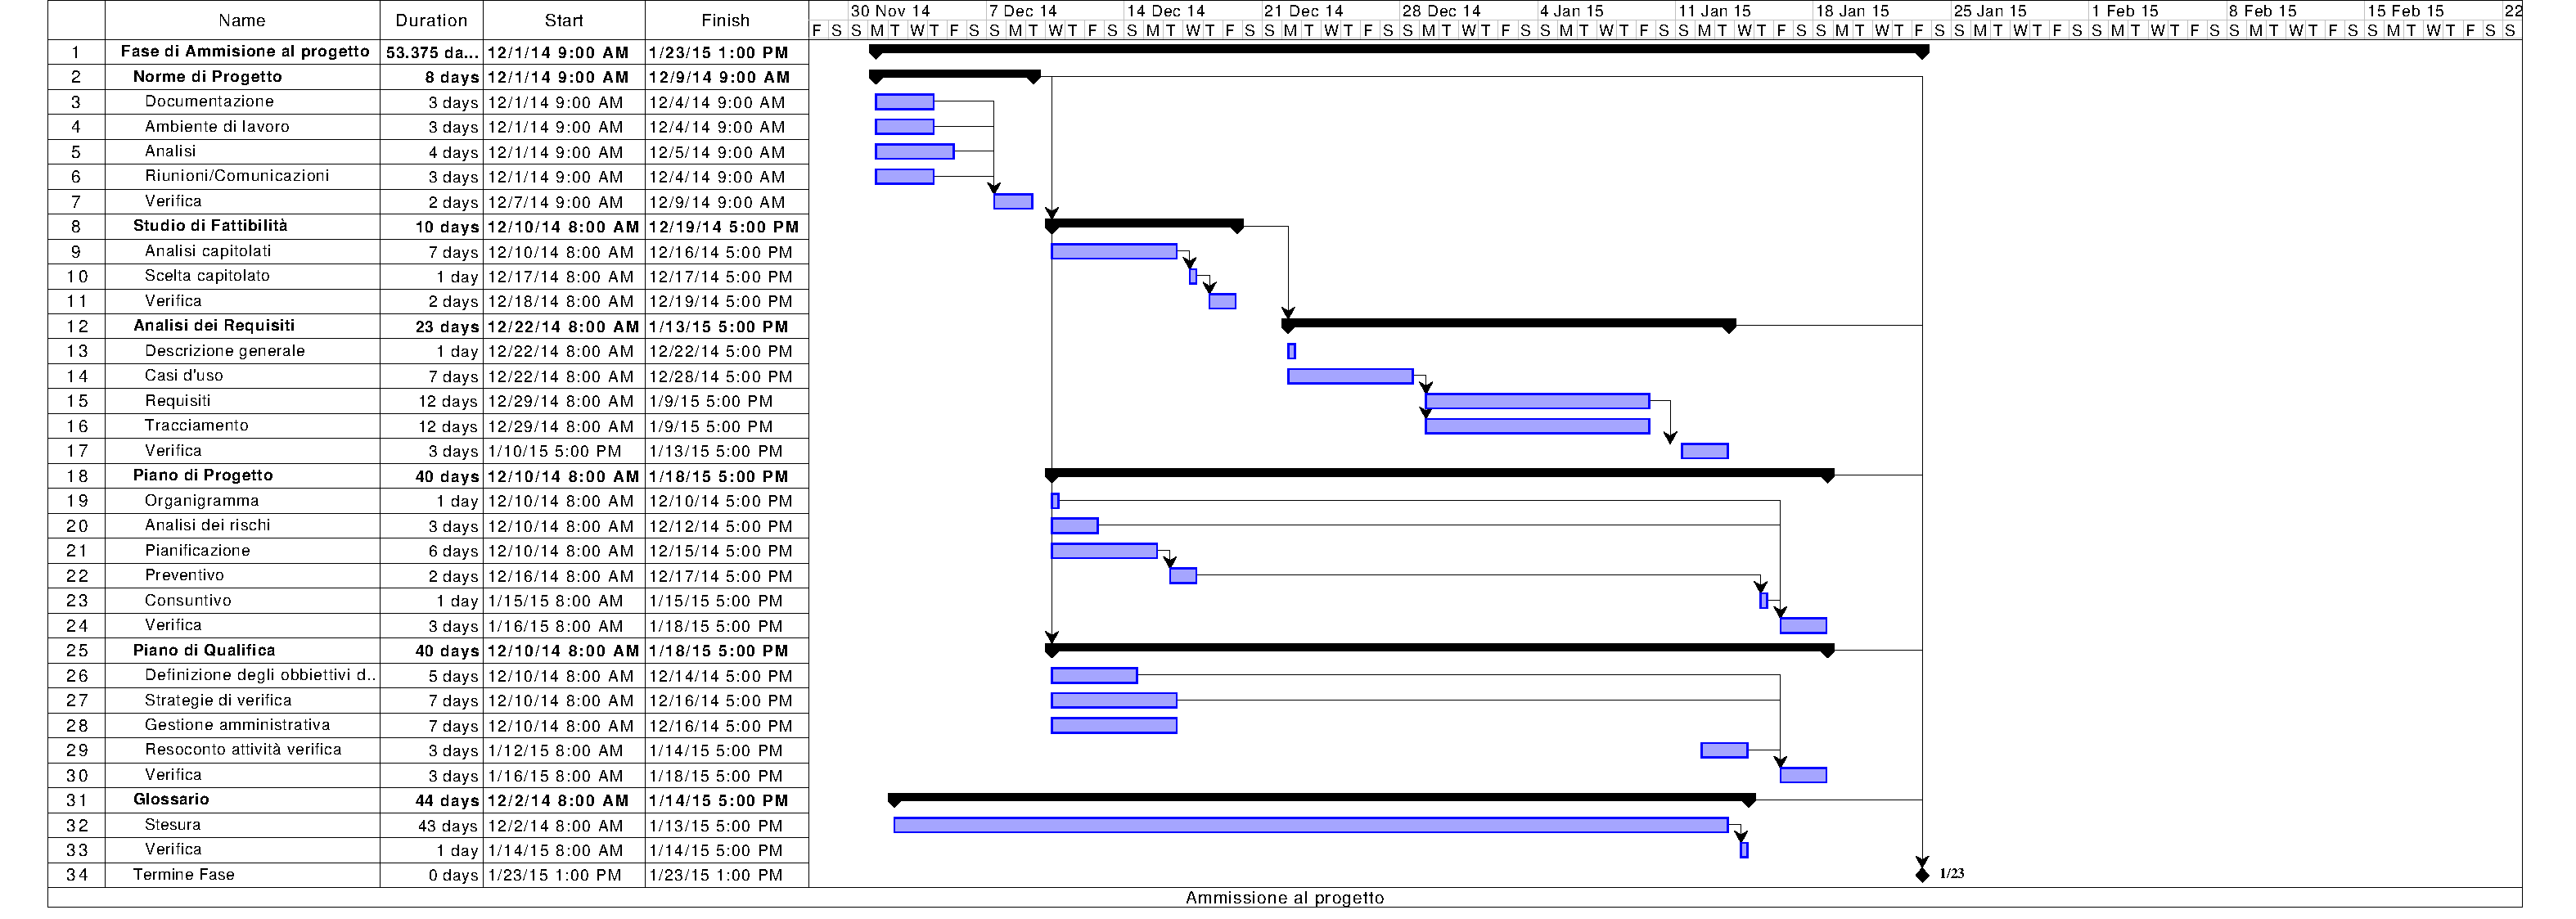
\includegraphics[width=23cm,height=10cm]{../immagini/gantt/ammissioneL.pdf}
\caption{Diagramma di Gantt - Fase di \fAt}\label{fig:ganttFA}
\end{figure}
\end{landscape}
\FloatBarrier
\subsection{\fADt}
\textbf{Periodo:} dal 2015-02-17 al 2015-03-08 \\
Questa fase inizia subito dopo la \RR e termina con l'inizio della fase di \fPA.\\
Lo scopo di questa fase è incrementare i vari documenti con quanto emerso dalla \RR e aggiungere eventuali requisiti che non sono stati individuati nella fase di \fA. \\
Durante questa fase vengono svolte le seguenti attività:
\begin{itemize}
\item \textbf{Incremento e verifica:} partendo dalle informazioni ricevute dalla \RR vengono incrementati e verificati i seguenti documenti: \AR, \NP, \PP, \G, e \PQ.
\end{itemize}
%\newpage
%\begin{landscape}
\subsubsection{Diagramma di Gantt delle attività}
\begin{figure}[h]
\centering
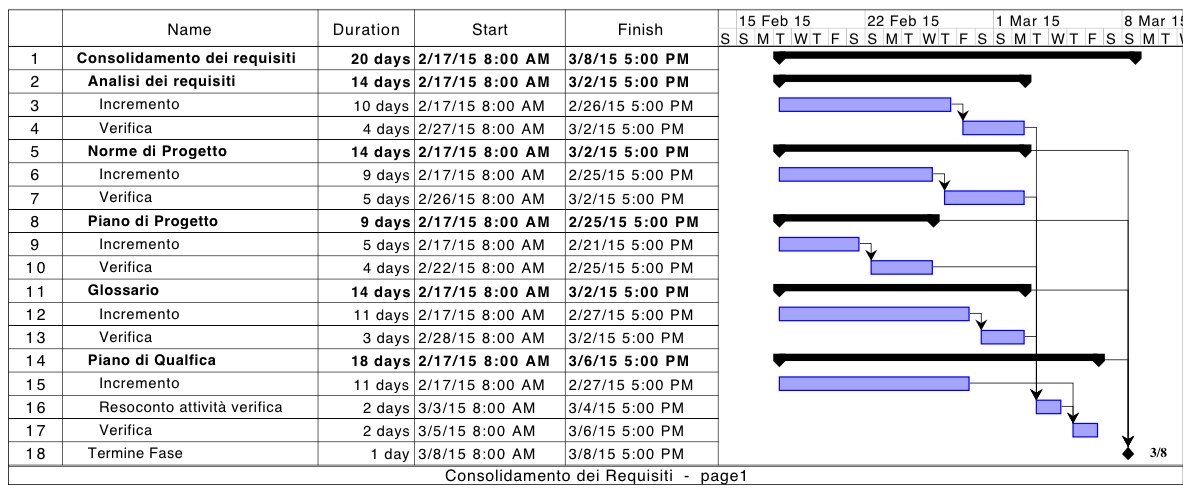
\includegraphics[width=\textwidth,keepaspectratio]{../immagini/gantt/consolidamentoRequisitiP.png}
\caption{Diagramma di Gantt - Fase di \fADt}\label{fig:ganttFAD}
\end{figure}
%\end{landscape}
\FloatBarrier
\subsection{\fPAt}\label{pAr}
\textbf{Periodo:} dal 2015-03-09 al 2015-03-29 \\
Questa fase inizia subito dopo \fAD e termina con l'inizio di \fPD: nel caso la fase precedente termini prima del previsto la data d'inizio di \fAD sarà anticipata.\\
Lo scopo di questa fase è definire l'architettura di alto livello della soluzione proposta. \\
La \gloxy{milestone} fissata a fine fase corrisponde ad una riunione con il \gloxy{proponente} per convalidare il lavoro svolto fino a questo punto.
Durante questa fase vengono svolte le seguenti attività:
\begin{itemize}
\item \textbf{Specifica Tecnica:} i \rPs redigono la \ST, documento che definisce la struttura ad alto livello della soluzione.
Questo documento definirà le tecnologie utilizzate, le componenti e le classi del sistema, il flusso di controllo dell'applicazione, i \gloxy{design pattern} utilizzati e il tracciamento dei requisiti;
\item \textbf{Incremento e verifica:} vengono incrementati e verificati i seguenti documenti: \NP, \G, \PP e \PQ.
\end{itemize}
\newpage
%\begin{landscape}
\subsubsection{Diagramma di Gantt delle attività}
\begin{figure}[h]
\centering
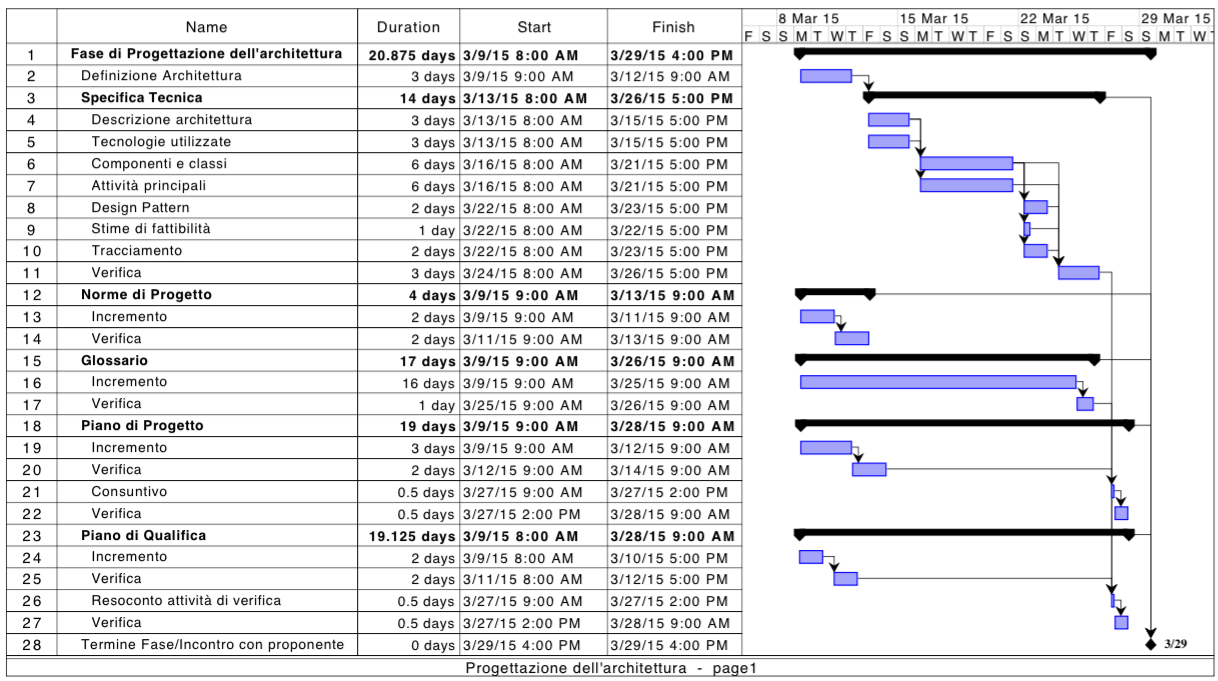
\includegraphics[width=\textwidth,keepaspectratio]{../immagini/gantt/progettazioneArchitetturaP.png}
\caption{Diagramma di Gantt - Fase di \fPAt}\label{fig:ganttFPA}
\end{figure}
%\end{landscape}
\FloatBarrier
\subsection{\fPDt}\label{progComponenti}
\textbf{Periodo:} dal 2015-03-30 al 2015-04-20 \\
Questa fase inizia subito dopo la fase \fPA e termina il 2015-04-20, la data di consegna della \RP, cioè 8 giorni prima dell'effettivo giorno di revisione.\\
Lo scopo di questa fase è di definire in modo preciso e non ambiguo i dettagli implementativi della soluzione. \\
Durante questa fase vengono svolte le seguenti attività:
\begin{itemize}
\item \textbf{Definizione del Prodotto:} partendo dalla \ST, i \rPs definiscono in modo più approfondito la struttura e le relazioni delle varie componenti della soluzione nel documento \DP;
\item \textbf{Incremento e Verifica:} vengono incrementati e verificati i seguenti documenti: \ST, \NP, \G, \PP e \PQ.
\end{itemize}
\newpage
%\begin{landscape}
\subsubsection{Diagramma di Gantt delle attività}
\begin{figure}[h]
\centering
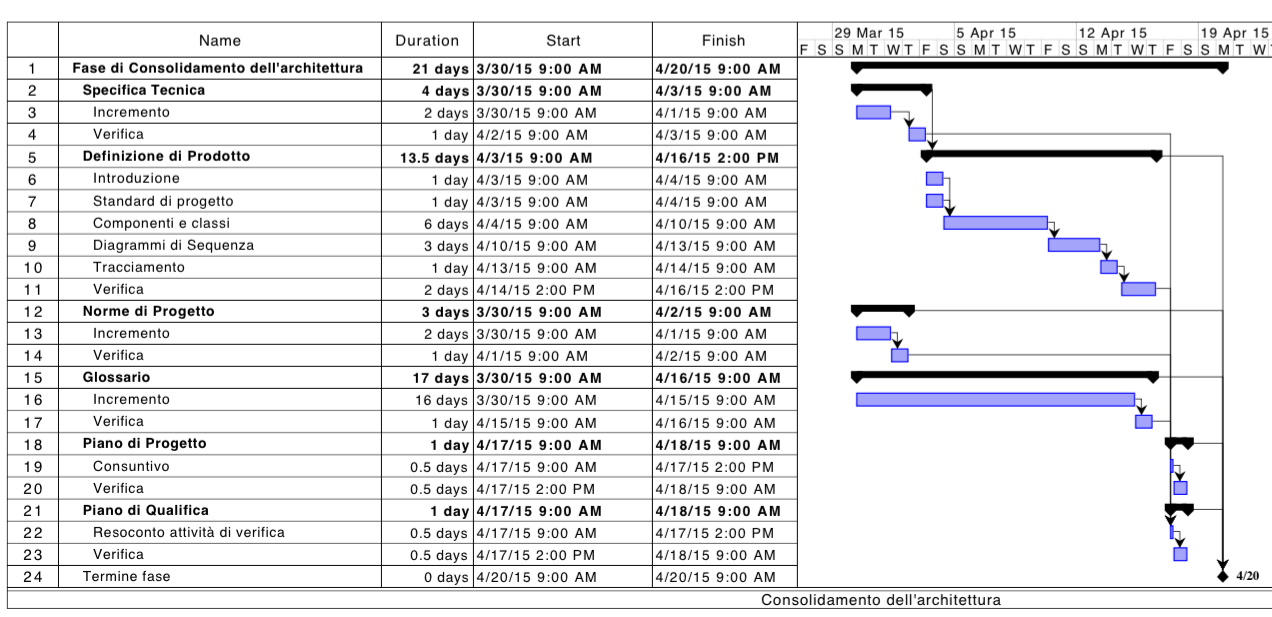
\includegraphics[width=\textwidth,keepaspectratio]{../immagini/gantt/consolidamentoArchitetturaP.png}
\caption{Diagramma di Gantt - Fase di \fPDt}\label{fig:ganttFPD}
\end{figure}
%\end{landscape}
\FloatBarrier
\subsection{\fCt}\label{cod}
\textbf{Periodo:} dal 2015-04-30 al 2015-05-24 \\
Questa fase inizia dopo la fase \fPD e termina 5 giorni prima della \RQ.
Lo scopo di questa fase è consolidare la \DP sulla base degli esiti della \RP, implementare la soluzione modellata e di redigere il \MU. \\
Ad inizio fase è stato fissato un incontro con il \gloxy{proponente} per presentare la soluzione definitiva ed avere un riscontro prima di iniziare l'attività di codifica. \\
Prima della fine di questa fase è stata fissata una \gloxy{milestone} coincidente ad una dimostrazione di prototipo al \gloxy{proponente}.
Durante questa fase vengono svolte le seguenti attività:
\begin{itemize}
\item \textbf{Codifica:} viene implementata la soluzione descritta nella \DP;
\item \textbf{Analisi del codice}: verrà eseguita in parallelo all'attività di codifica attraverso degli strumenti predisposti dall'amministratore (quali ad esempio script automatici) per garantire la consistenza e la correttezza del codice prodotto;
\item \textbf{Manuale Utente:} parallelamente all'implementazione della soluzione i \rps redigono il \MU. Tale documento fornirà le linee guida per l'utilizzo dell'applicazione da parte degli utenti;
\item \textbf{Incremento e verifica:} vengono incrementati e verificati tutti i documenti sulla base dell'esito della \RP.
\end{itemize}
\newpage
%\begin{landscape}
\subsubsection{Diagramma di Gantt delle attività}
\begin{figure}[h]
\centering
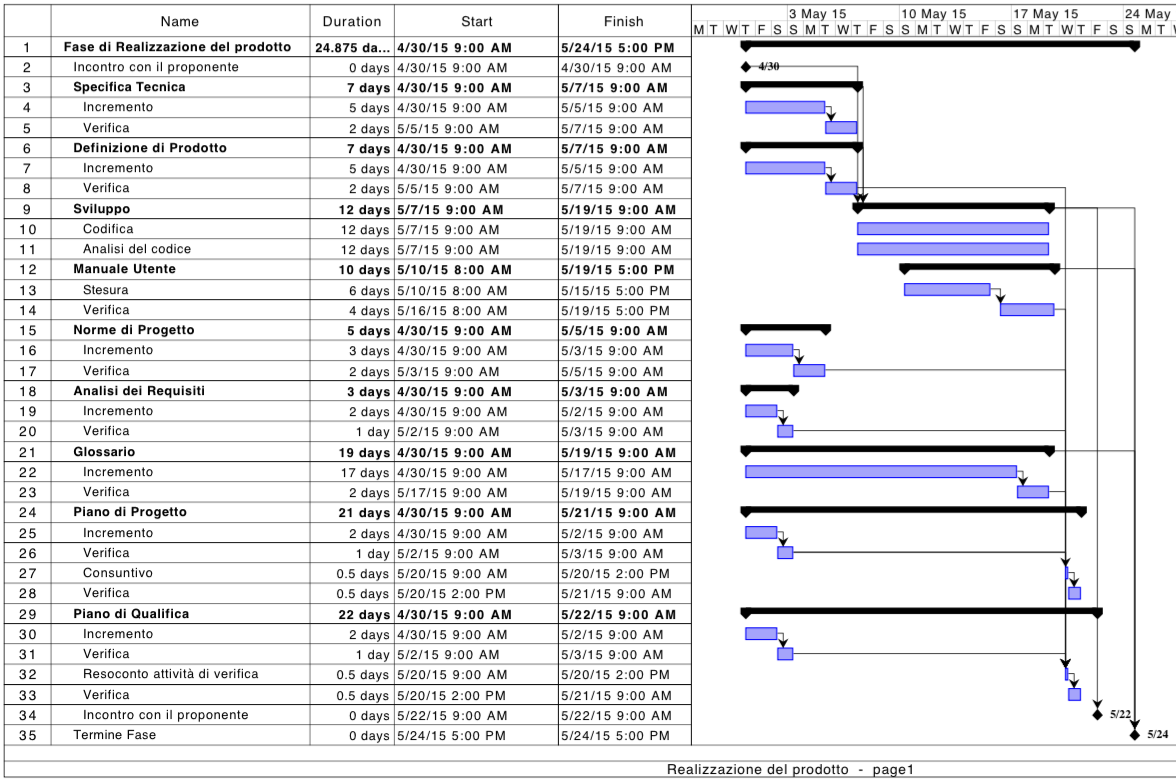
\includegraphics[width=\textwidth,keepaspectratio]{../immagini/gantt/realizzazioneProdottoP.png}
\caption{Diagramma di Gantt - Fase di \fCt}\label{fig:ganttFC}
\end{figure}
%\end{landscape}
\FloatBarrier
\subsection{\fVVt}\label{col}
\textbf{Periodo:} dal 2015-05-30 al 2015-06-10\\
Questa fase inizia dopo la \RQ e termina 8 giorni prima della \RA.\\
Tale fase rappresenta la conclusione delle varie attività di verifica realizzate nei singoli processi del ciclo di vita.\\
Durante questa fase il prodotto viene dapprima verificato, poi validato e successivamente testato. \\
Il prodotto verrà testato, oltre che dai componenti del gruppo, anche da utenti tester che saranno successivamente intervistati per dare un loro giudizio sul prodotto. \\
In questo modo il \gloxy{team} potrà avere un'idea di quanto realmente il prodotto realizzato possa essere interessante per il target di utenza identificato in fase di \AR.
Il termine della fase \fVVt coinciderà con una dimostrazione del prototipo al \gloxy{proponente}. \\
Le attività principali di questa fase sono:
\begin{itemize}
\item \textbf{Verifica del software:} il software realizzato viene verificato per garantirne la consistenza, la completezza e la correttezza;
\item \textbf{Validazione del software:} accerta, tramite tracciamento, che il prodotto sia conforme alle attese e soddisfi quindi i requisiti indicati in \analisiDeiRequisiti;
\item \textbf{Collaudo del software:} vengono testate le funzionalità offerte dal software;
\item \textbf{Incremento e verifica:} vengono incrementati e verificati tutti i documenti sulla base dell'esito della \RQ.
\end{itemize}
\newpage
%\begin{landscape}
\subsubsection{Diagramma di Gantt delle attività}
\begin{figure}[h]
\centering
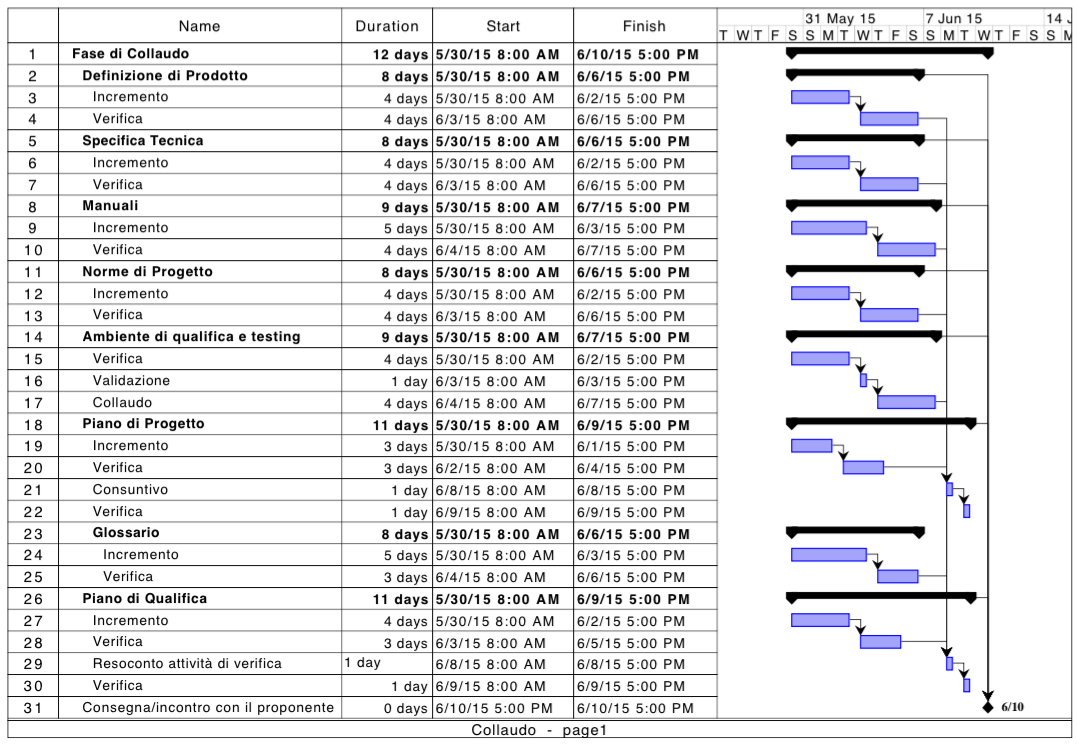
\includegraphics[width=\textwidth,keepaspectratio]{../immagini/gantt/collaudoP.png}
\caption{Diagramma di Gantt - Fase di \fVVt}\label{fig:ganttFVV}
\end{figure}
%\end{landscape}
\FloatBarrier
